%% abtex2-modelo-trabalho-academico.tex, v-1.9.2 laurocesar
%% Copyright 2012-2014 by abnTeX2 group at http://abntex2.googlecode.com/ 
%%
%% This work may be distributed and/or modified under the
%% conditions of the LaTeX Project Public License, either version 1.3
%% of this license or (at your option) any later version.
%% The latest version of this license is in
%%   http://www.latex-project.org/lppl.txt
%% and version 1.3 or later is part of all distributions of LaTeX
%% version 2005/12/01 or later.
%%
%% This work has the LPPL maintenance status `maintained'.
%% 
%% The Current Maintainer of this work is the abnTeX2 team, led
%% by Lauro César Araujo. Further information are available on 
%% http://abntex2.googlecode.com/
%%
%% This work consists of the files abntex2-modelo-trabalho-academico.tex,
%% abntex2-modelo-include-comandos and abntex2-modelo-references.bib
%%

% ------------------------------------------------------------------------
% ------------------------------------------------------------------------
% abnTeX2: Modelo de Trabalho Academico (tese de doutorado, dissertacao de
% mestrado e trabalhos monograficos em geral) em conformidade com 
% ABNT NBR 14724:2011: Informacao e documentacao - Trabalhos academicos -
% Apresentacao
% MODELO MODIFICADO PARA ATENDER AS ESPECIFICIDADES DO CURSO DE CIÊNCIA DA COMPUTAÇÃO DA UNIVERSIDADE ESTADUAL DO PIAUI
% ------------------------------------------------------------------------
% 

\documentclass[
	% -- opções da classe memoir --
	12pt,				% tamanho da fonte
	openright,			% capítulos começam em pág. ímpar (insere página vazia caso preciso)
	oneside,			% para impressão em verso e anverso. Oposto a oneside
	a4paper,			% tamanho do papel. 
	% -- opções da classe abntex2 --
	chapter=TITLE,		% títulos de capítulos convertidos em letras maiúsculas
	%section=TITLE,		% títulos de seções convertidos em letras maiúsculas
	%subsection=TITLE,	% títulos de subseções convertidos em letras maiúsculas
	%subsubsection=TITLE,% títulos de subsubseções convertidos em letras maiúsculas
	% -- opções do pacote babel --
	english,			% idioma adicional para hifenização
	%french,				% idioma adicional para hifenização
	%spanish,			% idioma adicional para hifenização
	brazil,				% o último idioma é o principal do documento
	]{abntex2}
% ---
% Pacotes básicos 
% ---
%\usepackage{lmodern}			% Usa a fonte Latin Modern	
\usepackage{mathptmx}
\renewcommand{\ABNTEXchapterfont}{\normalfont}
%\usepackage{bookman}		
\usepackage[T1]{fontenc}		% Selecao de codigos de fonte.
\usepackage[utf8]{inputenc}		% Codificacao do documento (conversão automática dos acentos)
\usepackage{lastpage}			% Usado pela Ficha catalográfica
\usepackage{indentfirst}		% Indenta o primeiro parágrafo de cada seção.
\usepackage{color}				% Controle das cores
\usepackage{graphicx}			% Inclusão de gráficos
\usepackage{microtype} 			% para melhorias de justificação
%\usepackage{geometry}
%\geometry{a4paper, left=3cm, right=2cm, bottom=2cm, top=3cm}
% ---
\graphicspath{ {./figs/} }
% ---
% Pacotes adicionais, usados apenas no âmbito do Modelo Canônico do abnteX2
% ---
\usepackage{lipsum}				% para geração de dummy text
% ---
% Pacotes de citações
% ---
\usepackage[brazilian,hyperpageref]{backref}	 % Paginas com as citações na bibl
\usepackage[alf]{abntex2cite}	% Citações padrão ABNT

% --- 
% CONFIGURAÇÕES DE PACOTES
% --- 

% ---
% Configurações do pacote backref
% Usado sem a opção hyperpageref de backref
\renewcommand{\backrefpagesname}{Citado na(s) página(s):~}
% Texto padrão antes do número das páginas
\renewcommand{\backref}{}
% Define os textos da citação
\renewcommand*{\backrefalt}[4]{
	\ifcase #1 %
		Nenhuma citação no texto.%
	\or
		Citado na página #2.%
	\else
		Citado #1 vezes nas páginas #2.%
	\fi}%
% ---

% ---
% Informações de dados para CAPA e FOLHA DE ROSTO
% ---
\titulo{TITULO DO SEU TRABALHO}
\autor{Nome do Aluno Completo}
\local{Teresina}
\data{2021}
\orientador{Nome do Orientador Completo}
\instituicao{Universidade Estadual do Piauí}
\tipotrabalho{Monografia (Graduação)}
% O preambulo deve conter o tipo do trabalho, o objetivo, o nome da instituição e a área de concentração 
\preambulo{Monografia submetida à Universidade Estadual do Piauí como parte dos requisitos para a obtenção do grau de Bacharel em Ciência da Computação.}




% Configurações de aparência do PDF final
%\definecolor{blue}{RGB}{41,5,195}
% informações do PDF
\makeatletter
\hypersetup{
     	%pagebackref=true,
		pdftitle={\@title}, 
		pdfauthor={\@author},
    	pdfsubject={\imprimirpreambulo},
	    pdfcreator={LaTeX with abnTeX2},
		pdfkeywords={abnt}{latex}{abntex}{abntex2}{trabalho acadêmico}, 
		colorlinks=true,       		% false: boxed links; true:              colored links
    	linkcolor=black,          	% color of internal links
    	citecolor=black,        		% color of links to bibliography
    	filecolor=magenta,      		% color of file links
		urlcolor=black,
		bookmarksdepth=4}

\makeatother
% --- 
% Espaçamentos entre linhas e parágrafos 
% --- 
% O tamanho do parágrafo é dado por:
\setlength{\parindent}{1.3cm}
% Controle do espaçamento entre um parágrafo e outro:
\setlength{\parskip}{0.2cm}  % tente também \onelineskip
% ---
% compila o indice
% ---
\makeindex
% ---

% --------------------------------------------------------------------------------------------------------
% % Início do documento
% --------------------------------------------------------------------------------------------------------
\begin{document}

% Retira espaço extra obsoleto entre as frases.
\frenchspacing 

% Capa
%---------------------------------------------------------------------------------------------------------

    \begin{center}
    {\ABNTEXchapterfont\large UNIVERSIDADE ESTADUAL DO PIAUÍ}\\
    {\ABNTEXchapterfont\large CIÊNCIA DA COMPUTAÇÃO}
    
    \vspace*{\fill}\vspace*{\fill}
    {\ABNTEXchapterfont\large \imprimirautor}  
    \vspace*{\fill}
   
    \vspace*{\fill}\vspace*{\fill}
    \begin{center}
    \ABNTEXchapterfont \bfseries \Large \imprimirtitulo
    \end{center}
    \vspace*{\fill}\vspace*{\fill}
   
  
   \end{center}  

      
    \begin{center}
    \vspace*{0.5cm}
    {\ABNTEXchapterfont\large TERESINA}
    \par
    {\ABNTEXchapterfont\large \imprimirdata}
    \vspace*{1cm}
    \end{center}
%--------------------------------------------------x------------------------------------------------------




% Folha de Rosto
% --------------------------------------------------------------------------------------------------------
\begin{folhaderosto}

  \begin{center}
    {\ABNTEXchapterfont\large \imprimirautor}

    \vspace*{\fill}\vspace*{\fill}
    \begin{center}
      \ABNTEXchapterfont\bfseries\Large \imprimirtitulo
    \end{center}
    \vspace*{\fill}
    
    \hspace{.45\textwidth}
    \begin{minipage}{.5\textwidth}
        \imprimirpreambulo
    \end{minipage}%
    \vspace*{\fill}
   \end{center}  

     \begin{center}
    \vspace*{0.5cm}
    {\ABNTEXchapterfont\large TERESINA}
    \par
    {\ABNTEXchapterfont\large \imprimirdata}
    \vspace*{1cm}
    \end{center}
  
\end{folhaderosto}
%--------------------------------------------------x------------------------------------------------------

% Folha ficha Catalográfica
% --------------------------------------------------------------------------------------------------------


\begin{fichacatalografica}
	\vspace*{\fill}					% Posição vertical
	\hrule							% Linha horizontal
	\begin{center}					% Minipage Centralizado
	\begin{minipage}[c]{12.5cm}		% Largura
	
	\imprimirautor
	
	\hspace{0.5cm} 
	{\imprimirtitulo / \imprimirautor. --	\imprimirlocal~~-- PI, Brasil, \imprimirdata.}
	
	{\hspace{0.5cm}\imprimirorientadorRotulo~\imprimirorientador}
	
	\hspace{0.5cm}\parbox[t]{\textwidth}{\imprimirtipotrabalho~--~\imprimirinstituicao, \imprimirdata.}

    \hspace{0.5cm}
		1. Embarcado.
		2. GSM.
        3. GPS.
        3. RF 433 Mhz.
		I. Nome do Orientador.
		II. Universidade Estadual do Piauí.
		 			
%\hspace{8.75cm} CDU 02:141:005.7\\
	
	\end{minipage}
	\end{center}
	\hrule
\end{fichacatalografica}
%--------------------------------------------------x------------------------------------------------------

% Folha de Aprovação
% --------------------------------------------------------------------------------------------------------

\begin{folhadeaprovacao}

  \begin{center}
    {\ABNTEXchapterfont\bfseries\Large \imprimirtitulo}\\
    \vspace*{\fill}
    {\ABNTEXchapterfont\large \imprimirautor}
    
    \vspace*{\fill}\vspace*{\fill}
    \hspace{.45\textwidth}
    \begin{minipage}{.5\textwidth}
        \imprimirpreambulo
    \end{minipage}%
    \vspace*{\fill}
   
   \ABNTEXchapterfont     
   {Trabalho aprovado. Teresina, 14 de Janeiro de \imprimirdata}
   \end{center}
   

   \assinatura{\textbf{\imprimirorientador} \\ Orientador} 
   \assinatura{\textbf{Nome do Avaliador-1 Completo} \\ }
   \assinatura{\textbf{Nome do Avaliador-2 Completo} \\ }

  
\end{folhadeaprovacao}
%--------------------------------------------------x------------------------------------------------------


% Dedicatória
%---------------------------------------------------------------------------------------------------------
\begin{dedicatoria}
  \vspace*{\fill}
   \centering
   \noindent
   \textit{ Este trabalho é dedicado às crianças adultas que,\\
   quando pequenas, sonharam em se tornar cientistas.} 
   \vspace*{\fill}
\end{dedicatoria}
%--------------------------------------------------x------------------------------------------------------

% Agradecimentos
% --------------------------------------------------------------------------------------------------------
\begin{agradecimentos}
\ABNTEXchapterfont
Nesta página deve constar o agradecimento àquelas pessoas e/ou instituições que marcaram de forma significativa a realização do seu trabalho. Segue exemplo:

Agradeço à Deus pela minha vida e pela vida de todas as pessoas que fazem parte dela.

A minha mãe e meu pai por me incentivarem a cada dia a alcançar meus sonhos, paciência, amor e suporte na minha árdua caminha até aqui.

A professora Fulana de Tal por me orientar e me guiar nessas últimas etapas do curso.

Aos colegas de curso que compartilharam conhecimento e bons momentos durante minha jornada na UESPI.

Ao amigo Ciclano de Tal por todo suporte e contribuição na realização deste trabalho.

A todos que direta ou indiretamente fizeram parte da minha formação, \textit{"thank you guys"}.

\end{agradecimentos}
%--------------------------------------------------x------------------------------------------------------

% Epígrafe
% --------------------------------------------------------------------------------------------------------
\begin{epigrafe}
    \vspace*{\fill}
	\begin{flushright}
		\textit{``A arma mais forte em dois milhões de anos\\
		de história humana: tecnologia de comunicação.`` \\
		(Inagaki, Riichiro; Dr. Stone, 2019)\\.}
	\end{flushright}
\end{epigrafe}
%--------------------------------------------------x------------------------------------------------------


% Resumo
%---------------------------------------------------------------------------------------------------------
\setlength{\absparsep}{18pt} % ajusta o espaçamento dos parágrafos do resumo
\begin{resumo}
\ABNTEXchapterfont
Consiste na apresentação dos pontos relevantes de um texto. O resumo deve dar uma visão rápida e clara do trabalho; constitui-se em uma sequencia de frases concisas e objetivas e não de uma simples enumeração de tópicos. Apresenta os objetivos do estudo, o problema, a metodologia, resultados alcançados e conclusão. Deve ser digitado em espaço simples e sem parágrafos, não ultrapassando a 500 palavras.


\textbf{Palavras-chaves}:Palavra-1. Palavra-2. Palavra-3.
\end{resumo}
%--------------------------------------------------x------------------------------------------------------


% Abstract
%---------------------------------------------------------------------------------------------------------
\begin{resumo}[Abstract]
\ABNTEXchapterfont
Consiste em traduzir o texto do resumo para o idioma ingles.

% \begin{otherlanguage*}{english}
%   This is the english abstract.
%   \vspace{\onelineskip}
%   \noindent 

\textbf{Key-words}: Bla bla bla. Word-2. Word-3.
\end{resumo}
%--------------------------------------------------x------------------------------------------------------


% inserir lista de ilustrações
%---------------------------------------------------------------------------------------------------------
\pdfbookmark[0]{\listfigurename}{lof}
\listoffigures*
\cleardoublepage
%--------------------------------------------------x------------------------------------------------------


% inserir lista de tabelas
%---------------------------------------------------------------------------------------------------------
\pdfbookmark[0]{\listtablename}{lot}
\listoftables*
\cleardoublepage
%--------------------------------------------------x------------------------------------------------------


% inserir lista de abreviaturas e siglas
%---------------------------------------------------------------------------------------------------------
\begin{siglas}
\ABNTEXchapterfont\item[TCP] Protocolo de Controle de Transmissão
\item[UDP] Protocolo de Datagrama do Usuário 
\item[VoIP] Voz sobre IP 
\item[RTP] Protocolo Transporte em Tempo Real
\item[MPRTP] Protocolo de Transporte em Tempo Real de Caminho Multiplos \item[RTCP] Protocolo de Controle de Transporte em Tempo Real
\item[MPTCP] Protocolo de Controle de Transporte de Caminho Multiplo 
\end{siglas}
%--------------------------------------------------x------------------------------------------------------
\pdfbookmark[0]{\contentsname}{toc}
\tableofcontents*
\cleardoublepage
\textual
%--------------------------------------------------x------------------------------------------------------


                                            % INTRODUÇÃO %
%---------------------------------------------------------------------------------------------------------
\chapter{Introdução}
\ABNTEXchapterfont
Esta seção delimita o assunto, apresenta brevemente os objetivos do trabalho e as razões de sua elaboração, bem como as relações existentes com outros trabalhos. Descreve o problema e as questões norteadoras ou hipóteses. Não deve antecipar conclusões e recomendações.

Lorem ipsum dolor sit amet, consectetur adipiscing elit. Nullam congue purus sit amet dolor finibus, sit amet mattis lacus fermentum. Maecenas vel sagittis risus. Ut sit amet mauris magna.\cite{wu2001streaming}. Nullam congue purus sit amet dolor finibus, sit amet mattis lacus fermentum. Maecenas vel sagittis risus. Ut sit amet mauris magna.\cite{mao2006mrtp}



%--------------------------------------------------x------------------------------------------------------

                                            % JUSTIFICATIVA %
%---------------------------------------------------------------------------------------------------------
\chapter{Justificativa}
Ressalte a importância do tema proposto e a necessidade de um estudo mais aprofundado. Utilize  argumentos objetivos e citações de autores reconhecidos nessa area de pesquisa.

Quisque ac eros arcu. Nulla vestibulum gravida turpis, a convallis mauris tristique quis. Morbi iaculis vulputate lacus tincidunt facilisis. Phasellus sit amet velit non libero molestie feugiat ut eget justo. Sed fringilla volutpat ligula, vel pharetra tellus congue quis. Phasellus et justo eu tellus viverra suscipit eu nec ipsum. Pellentesque arcu ante, rutrum auctor diam ut, rhoncus cursus ipsum. Nullam gravida, ante quis aliquet lobortis, magna lectus porta turpis, eget elementum dui odio ac elit. In sagittis, lorem sed tempus eleifend, eros diam congue quam, sed posuere quam ipsum sit amet enim.\cite{ahsan2011multipath}

Maecenas ac lectus et arcu vestibulum hendrerit ac ac nulla. Nulla non ornare nibh. Morbi elementum hendrerit semper. Nullam consectetur euismod eros eget egestas. Donec magna libero, lacinia id viverra laoreet, commodo ac augue. Vestibulum dictum dolor et porta dapibus. Suspendisse potenti.\footnote{https://sharelink.tv/welcome} e o CoreCloud\footnote{https://corecloud.tv/}  Maecenas ac lectus et arcu vestibulum hendrerit ac ac nulla. Nulla non ornare nibh. Morbi elementum hendrerit semper. Nullam consectetur euismod eros eget egestas.

Integer at ante eros. Etiam tincidunt posuere feugiat. Praesent eget egestas eros. Proin vitae risus ultrices, laoreet libero fringilla, ultricies felis. Vestibulum tristique id ex vel feugiat. Donec convallis ut ligula eget laoreet. Aenean vehicula metus eget ante auctor, ac tempor dui blandit. Quisque sed nulla facilisis, semper mauris non, molestie dui.

%--------------------------------------------------x------------------------------------------------------

                                            % OBJETIVOS %
%---------------------------------------------------------------------------------------------------------
\chapter{Objetivos}
\section{Geral}
Nullam commodo augue ante, nec feugiat massa tristique id. Integer dolor odio, lacinia non pretium hendrerit, ullamcorper eu odio.


\section{Específico}
\begin{itemize}
\item Mauris vel sapien metus. Nulla feugiat justo vitae auctor efficitur. In hac habitasse platea dictumst. Donec rutrum iaculis enim sit amet vestibulum. Nullam aliquam felis nec augue eleifend finibus.
\item Vestibulum eleifend dictum aliquam. Phasellus rhoncus ex a est volutpat tincidunt.
\item Vestibulum eleifend dictum aliquam. Phasellus rhoncus ex a est volutpat tincidunt.
\item Vestibulum eleifend dictum aliquam. Phasellus rhoncus ex a est volutpat tincidunt.
\end{itemize} 
%--------------------------------------------------x------------------------------------------------------

                                          % METODOLOGIA %
%---------------------------------------------------------------------------------------------------------
\chapter{Metodologia}
It has survived not only fivecenturies, but also the leap into electronic typesetting, remaining essentially unchanged. It waspopularised in the 1960s with the release of Letraset sheets containing Lorem Ipsum passages,and more recently with desktop publishing software like Aldus PageMaker including versions of Lorem Ipsum.\cite{ahsan2016multipath}. It has survived not only fivecenturies, but also the leap into electronic typesetting, remaining essentially unchanged.

\begin{itemize}
\item ETAPA 1 - Lorem Ipsum is simply dummy text of the printing and typesetting industry. Lorem Ipsum hasbeen the industry’s standard dummy text ever since the 1500s, when an unknown printer tooka galley of type and scrambled it to make a type specimen book. It has survived not only fivecenturies, but also the leap into electronic typesetting, remaining essentially unchanged. It waspopularised in the 1960s with the release of Letraset sheets containing Lorem Ipsum passages,and more recently with desktop publishing software like Aldus PageMaker including versions of Lorem Ipsum. Resaltando os importantes trabalhos de \cite{ghareeb2008multiple} e \cite{afzal2019holistic}.
\item ETAPA 2 - Lorem Ipsum is simply dummy text of the printing and typesetting industry. Lorem Ipsum hasbeen the industry’s standard dummy text ever since the 1500s, when an unknown printer tooka galley of type and scrambled it to make a type specimen book. It has survived not only fivecenturies, but also the leap into electronic typesetting, remaining essentially unchanged. 
\item ETAPA 3 - Sed posuere diam turpis, at vulputate urna mollis in. Class aptent taciti sociosqu ad litora torquent per conubia nostra, per inceptos himenaeos. .
\item Lorem ipsum dolor sit amet, consectetur adipiscing elit. Nullam congue purus sit amet dolor finibus, sit amet mattis lacus fermentum. Maecenas vel sagittis risus. Ut sit amet mauris magna. Curabitur tristique accumsan diam, eget fermentum mauris mattis non. Integer eget libero at purus egestas condimentum. Mauris eleifend pulvinar varius. Mauris sed orci ac ligula semper tristique sed sit amet lacus. Vestibulum accumsan a sem ut elementum. Ut nec augue justo. Duis sed consequat ante. Aenean iaculis ligula eu turpis lacinia maximus. Integer iaculis interdum molestie. Nullam a rutrum arcu. Morbi finibus, nisi ac placerat fermentum, nisi ex condimentum lacus, ac tempus diam odio nec augue. Curabitur placerat elit augue, et tempus odio sagittis id.
\item ETAPA 5 - Sed posuere diam turpis, at vulputate urna mollis in. Class aptent taciti sociosqu ad litora torquent per conubia nostra, per inceptos himenaeos.
\end{itemize}

\section{Tecnologias Utilizadas}
\subsection{Framework}
Lorem Ipsum is simply dummy text of the printing and typesetting industry. Lorem Ipsum hasbeen the industry’s standard dummy text ever since the 1500s, when an unknown printer tooka galley of type and scrambled it to make a type specimen book. It has survived not only fivecenturies, but also the leap into electronic typesetting, remaining essentially unchanged. It waspopularised in the 1960s with the release of Letraset sheets containing Lorem Ipsum passages,and more recently with desktop publishing software like Aldus PageMaker including versions of Lorem Ipsum.\footnote{https://framewor.freedesktop.org/features/}

\subsection{UDP}
O User Datagram Protocol é um protocolo simples não orientado a conexões da camada de transporte. Definido pela RFC768\footnote{https://tools.ietf.org/html/rfc768} ele envia um  datagrama pela rede mas sem garantia de entrega, isso porque esse protocolo adota a heurística do melhor esforço para realizar a transações de pacotes entre dois computadores dentro de uma rede IPV4 ou IPV6.
 O protocolo UDP é a escolha adequada quando se deseja realizar a transmissão de um fluxo de dados em tempo real por não fazer uso da criação e destruição de conexões como faz o Protocolo de Controle de Transmissão - TCP, porque isso faria o tempo de transmissão dos dados aumentar e inviabilizaria o objetivo desse tipo transmissão. Entretanto o protocolo não trata perda de pacotes, retransmissão, controle de fluxo ou \textit{timeout} o que pode inviabilizar as transmissões devido a baixa qualidade dos dados recebidos, assim os protocolos apresentados posteriormente tratam esses problemas.

\subsection{RTP/RTCP}
Lorem Ipsum is simply dummy text of the printing and typesetting industry. Lorem Ipsum hasbeen the industry’s standard dummy text ever since the 1500s, when an unknown printer tooka galley of type and scrambled it to make a type specimen book. It has survived not only fivecenturies, but also the leap into electronic typesetting, remaining essentially unchanged. It waspopularised in the 1960s with the release of Letraset sheets containing Lorem Ipsum passages,and more recently with desktop publishing software like Aldus PageMaker including versions of Lorem Ipsum.\footnote{https://tools.ietf.org/html/rfc3550}.  A figura \ref{fig:gy80}  representa o funcionamento desses protocolos em um serviço de Voz sobre IP - VoIP.

\begin{figure}[!htb]
\begin{center}
\caption{Representação da utilização dos protocolos RTP e RTCP }
\label{fig:gy80}
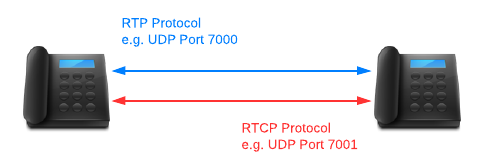
\includegraphics[width=0.6\linewidth]{rtp-rtcp.png}
\end{center}
\legend{Fonte: \cite{rtp-rtcp} }
\end{figure}

\subsection{Outro Protocolo}
Definido pela  \textit{draft} da IETF\footnote{https://tools.ietf.org/html/draft-ietf-avtcore-mprtp-03} Lorem Ipsum is simply dummy text of the printing and typesetting industry. Lorem Ipsum hasbeen the industry’s standard dummy text ever since the 1500s, when an unknown printer tooka galley of type and scrambled it to make a type specimen book. It has survived not only fivecenturies, but also the leap into electronic typesetting, remaining essentially unchanged. It waspopularised in the 1960s with the release of Letraset sheets containing Lorem Ipsum passages,and more recently with desktop publishing software like Aldus PageMaker including versions of Lorem Ipsum. \cite{herrero2017modeling} na figura \ref{fig:rtp-mprtp}.It waspopularised in the 1960s with the release of Letraset sheets containing Lorem Ipsum passages,and more recently with desktop publishing software like Aldus PageMaker including versions of Lorem Ipsum.\footnote{https://www.techopedia.com/definition/28190/5-tuple}. 

\begin{figure}[!htb]
\begin{center}
\caption{Representação da utilização dos protocolos RTP e RTCP }
\label{fig:rtp-mprtp}
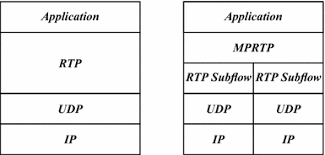
\includegraphics[width=0.6\linewidth]{rtp-mprtp.png}
\end{center}
\legend{Fonte: \cite{herrero2017modeling} }
\end{figure}

%--------------------------------------------------x-----------------------------------------------------
\chapter{Cronograma - (TCC 1)} 
As atividades futuras deveram o seguinte cronograma.

\begin{table}[h]
\centering
\caption{Cronograma}
\vspace{0.5cm}
\begin{tabular}{c|c|c|c|c|c|c}
\label{tabela-coleta}

Atividades&Fev&Mar&Abr&Mai&Jun&Jul\\
\hline 
Estudo  &X&X&&&\\
Implementação &X&X&X&X&\\
Teste de Avaliação e Comparação  &&&&X&X  \\
Escrita da Resultados  &&&&X&X& \\
Apresentação do Trabalho &&&&&&X   
\end{tabular}
\end{table}


%--------------------------------------------------x-----------------------------------------------------
\chapter{Resultados}
Lorem Ipsum is simply dummy text of the printing and typesetting industry. Lorem Ipsum hasbeen the industry’s standard dummy text ever since the 1500s, when an unknown printer tooka galley of type and scrambled it to make a type specimen book. It has survived not only fivecenturies, but also the leap into electronic typesetting, remaining essentially unchanged. It waspopularised in the 1960s with the release of Letraset sheets containing Lorem Ipsum passages,and more recently with desktop publishing software like Aldus PageMaker including versions of Lorem Ipsum.


%--------------------------------------------------x-----------------------------------------------------
\chapter{Considerações Finais}
Lorem Ipsum is simply dummy text of the printing and typesetting industry. Lorem Ipsum hasbeen the industry’s standard dummy text ever since the 1500s, when an unknown printer tooka galley of type and scrambled it to make a type specimen book. It has survived not only fivecenturies, but also the leap into electronic typesetting, remaining essentially unchanged. It waspopularised in the 1960s with the release of Letraset sheets containing Lorem Ipsum passages,and more recently with desktop publishing software like Aldus PageMaker including versions of Lorem Ipsum.


%{Referencias Bibliograficas}
%---------------------------------------------------------------------------------------------------------
\bibliography{biblio.bib}
\printindex

\end{document}
